% C3: Transform frequency heatmap (kernel x transform)
% Regenerated from results/augmentation/retest_post_session2.json
% 22 Rodinia kernels x 6 transforms, aggregated across L1-L4 and all API variants
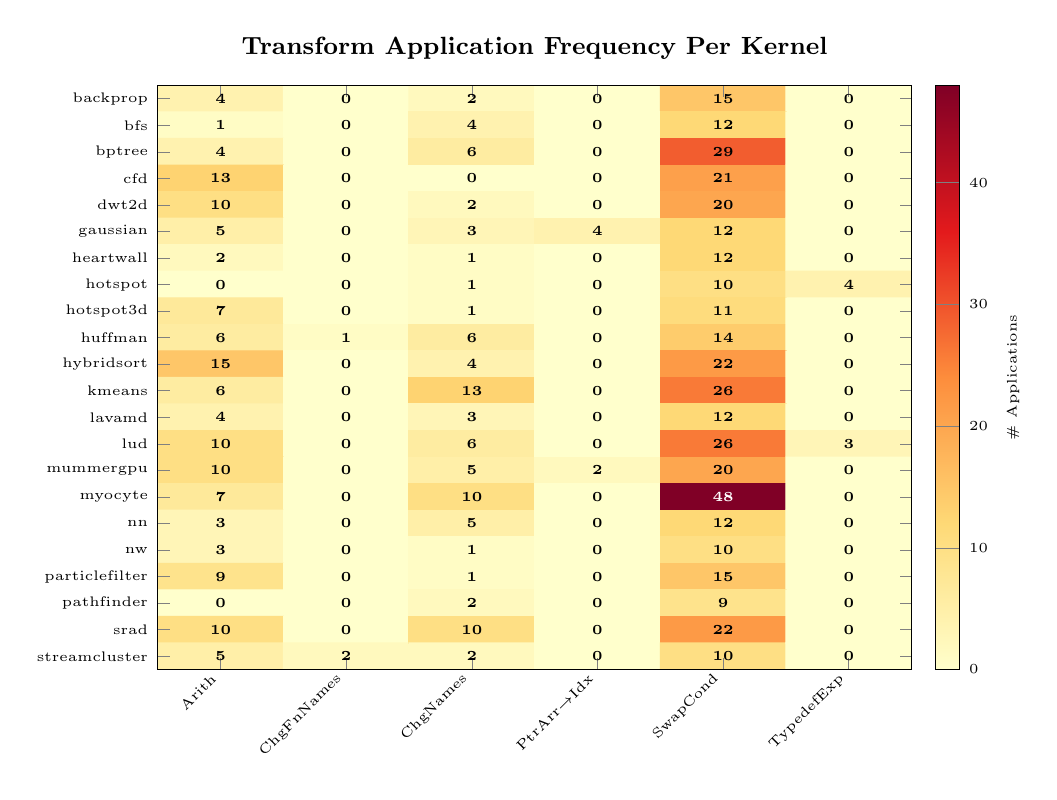
\begin{tikzpicture}
\begin{axis}[
  width=0.92\columnwidth,
  height=9cm,
  enlargelimits=false,
  axis on top,
  y dir=reverse,
  tick label style={font=\tiny},
  colorbar,
  colorbar style={
    font=\tiny, width=0.3cm,
    ylabel={\# Applications},
    ylabel style={font=\tiny},
  },
  colormap={ylOrRd}{
    rgb255(0)=(255,255,204)
    rgb255(14)=(254,217,118)
    rgb255(28)=(253,141,60)
    rgb255(42)=(227,26,28)
    rgb255(56)=(128,0,38)
  },
  point meta min=0, point meta max=48,
  xtick={0,...,5},
  xticklabels={Arith,ChgFnNames,ChgNames,{PtrArr{\ensuremath{\to}}Idx},SwapCond,TypedefExp},
  xticklabel style={font=\tiny, rotate=45, anchor=east},
  ytick={0,...,21},
  yticklabels={backprop,bfs,bptree,cfd,dwt2d,gaussian,heartwall,hotspot,hotspot3d,huffman,hybridsort,kmeans,lavamd,lud,mummergpu,myocyte,nn,nw,particlefilter,pathfinder,srad,streamcluster},
  yticklabel style={font=\tiny},
  xmin=-0.5, xmax=5.5,
  ymin=-0.5, ymax=21.5,
  title={Transform Application Frequency Per Kernel},
  title style={font=\small\bfseries},
]
  %% Color matrix
  \addplot[matrix plot*, mesh/cols=6, point meta=explicit] coordinates {
    (0,0)[4]  (1,0)[0]  (2,0)[2]  (3,0)[0]  (4,0)[15]  (5,0)[0]
    (0,1)[1]  (1,1)[0]  (2,1)[4]  (3,1)[0]  (4,1)[12]  (5,1)[0]
    (0,2)[4]  (1,2)[0]  (2,2)[6]  (3,2)[0]  (4,2)[29]  (5,2)[0]
    (0,3)[13]  (1,3)[0]  (2,3)[0]  (3,3)[0]  (4,3)[21]  (5,3)[0]
    (0,4)[10]  (1,4)[0]  (2,4)[2]  (3,4)[0]  (4,4)[20]  (5,4)[0]
    (0,5)[5]  (1,5)[0]  (2,5)[3]  (3,5)[4]  (4,5)[12]  (5,5)[0]
    (0,6)[2]  (1,6)[0]  (2,6)[1]  (3,6)[0]  (4,6)[12]  (5,6)[0]
    (0,7)[0]  (1,7)[0]  (2,7)[1]  (3,7)[0]  (4,7)[10]  (5,7)[4]
    (0,8)[7]  (1,8)[0]  (2,8)[1]  (3,8)[0]  (4,8)[11]  (5,8)[0]
    (0,9)[6]  (1,9)[1]  (2,9)[6]  (3,9)[0]  (4,9)[14]  (5,9)[0]
    (0,10)[15]  (1,10)[0]  (2,10)[4]  (3,10)[0]  (4,10)[22]  (5,10)[0]
    (0,11)[6]  (1,11)[0]  (2,11)[13]  (3,11)[0]  (4,11)[26]  (5,11)[0]
    (0,12)[4]  (1,12)[0]  (2,12)[3]  (3,12)[0]  (4,12)[12]  (5,12)[0]
    (0,13)[10]  (1,13)[0]  (2,13)[6]  (3,13)[0]  (4,13)[26]  (5,13)[3]
    (0,14)[10]  (1,14)[0]  (2,14)[5]  (3,14)[2]  (4,14)[20]  (5,14)[0]
    (0,15)[7]  (1,15)[0]  (2,15)[10]  (3,15)[0]  (4,15)[48]  (5,15)[0]
    (0,16)[3]  (1,16)[0]  (2,16)[5]  (3,16)[0]  (4,16)[12]  (5,16)[0]
    (0,17)[3]  (1,17)[0]  (2,17)[1]  (3,17)[0]  (4,17)[10]  (5,17)[0]
    (0,18)[9]  (1,18)[0]  (2,18)[1]  (3,18)[0]  (4,18)[15]  (5,18)[0]
    (0,19)[0]  (1,19)[0]  (2,19)[2]  (3,19)[0]  (4,19)[9]  (5,19)[0]
    (0,20)[10]  (1,20)[0]  (2,20)[10]  (3,20)[0]  (4,20)[22]  (5,20)[0]
    (0,21)[5]  (1,21)[2]  (2,21)[2]  (3,21)[0]  (4,21)[10]  (5,21)[0]
  };
  %% Black labels for light cells (value < 30)
  \addplot[
    only marks, mark=none, point meta=explicit,
    nodes near coords={\pgfmathfloattoint{\pgfplotspointmeta}\pgfmathresult},
    nodes near coords align={center},
    every node near coord/.style={font=\tiny\bfseries, text=black, inner sep=0pt}
  ] coordinates {
    (0,0)[4]  (1,0)[0]  (2,0)[2]  (3,0)[0]  (4,0)[15]  (5,0)[0]
    (0,1)[1]  (1,1)[0]  (2,1)[4]  (3,1)[0]  (4,1)[12]  (5,1)[0]
    (0,2)[4]  (1,2)[0]  (2,2)[6]  (3,2)[0]  (4,2)[29]  (5,2)[0]
    (0,3)[13]  (1,3)[0]  (2,3)[0]  (3,3)[0]  (4,3)[21]  (5,3)[0]
    (0,4)[10]  (1,4)[0]  (2,4)[2]  (3,4)[0]  (4,4)[20]  (5,4)[0]
    (0,5)[5]  (1,5)[0]  (2,5)[3]  (3,5)[4]  (4,5)[12]  (5,5)[0]
    (0,6)[2]  (1,6)[0]  (2,6)[1]  (3,6)[0]  (4,6)[12]  (5,6)[0]
    (0,7)[0]  (1,7)[0]  (2,7)[1]  (3,7)[0]  (4,7)[10]  (5,7)[4]
    (0,8)[7]  (1,8)[0]  (2,8)[1]  (3,8)[0]  (4,8)[11]  (5,8)[0]
    (0,9)[6]  (1,9)[1]  (2,9)[6]  (3,9)[0]  (4,9)[14]  (5,9)[0]
    (0,10)[15]  (1,10)[0]  (2,10)[4]  (3,10)[0]  (4,10)[22]  (5,10)[0]
    (0,11)[6]  (1,11)[0]  (2,11)[13]  (3,11)[0]  (4,11)[26]  (5,11)[0]
    (0,12)[4]  (1,12)[0]  (2,12)[3]  (3,12)[0]  (4,12)[12]  (5,12)[0]
    (0,13)[10]  (1,13)[0]  (2,13)[6]  (3,13)[0]  (4,13)[26]  (5,13)[3]
    (0,14)[10]  (1,14)[0]  (2,14)[5]  (3,14)[2]  (4,14)[20]  (5,14)[0]
    (0,15)[7]  (1,15)[0]  (2,15)[10]  (3,15)[0]  (5,15)[0]
    (0,16)[3]  (1,16)[0]  (2,16)[5]  (3,16)[0]  (4,16)[12]  (5,16)[0]
    (0,17)[3]  (1,17)[0]  (2,17)[1]  (3,17)[0]  (4,17)[10]  (5,17)[0]
    (0,18)[9]  (1,18)[0]  (2,18)[1]  (3,18)[0]  (4,18)[15]  (5,18)[0]
    (0,19)[0]  (1,19)[0]  (2,19)[2]  (3,19)[0]  (4,19)[9]  (5,19)[0]
    (0,20)[10]  (1,20)[0]  (2,20)[10]  (3,20)[0]  (4,20)[22]  (5,20)[0]
    (0,21)[5]  (1,21)[2]  (2,21)[2]  (3,21)[0]  (4,21)[10]  (5,21)[0]
  };
  %% White labels for dark cells (value >= 30)
  \addplot[
    only marks, mark=none, point meta=explicit,
    nodes near coords={\pgfmathfloattoint{\pgfplotspointmeta}\pgfmathresult},
    nodes near coords align={center},
    every node near coord/.style={font=\tiny\bfseries, text=white, inner sep=0pt}
  ] coordinates {
    (4,15)[48]
  };
\end{axis}
\end{tikzpicture}